% SOURCE: ../../edit-harness/results/frame_a/cells/cell_*_real_MIX_A_*.json
% !TEX encoding = UTF-8 Unicode
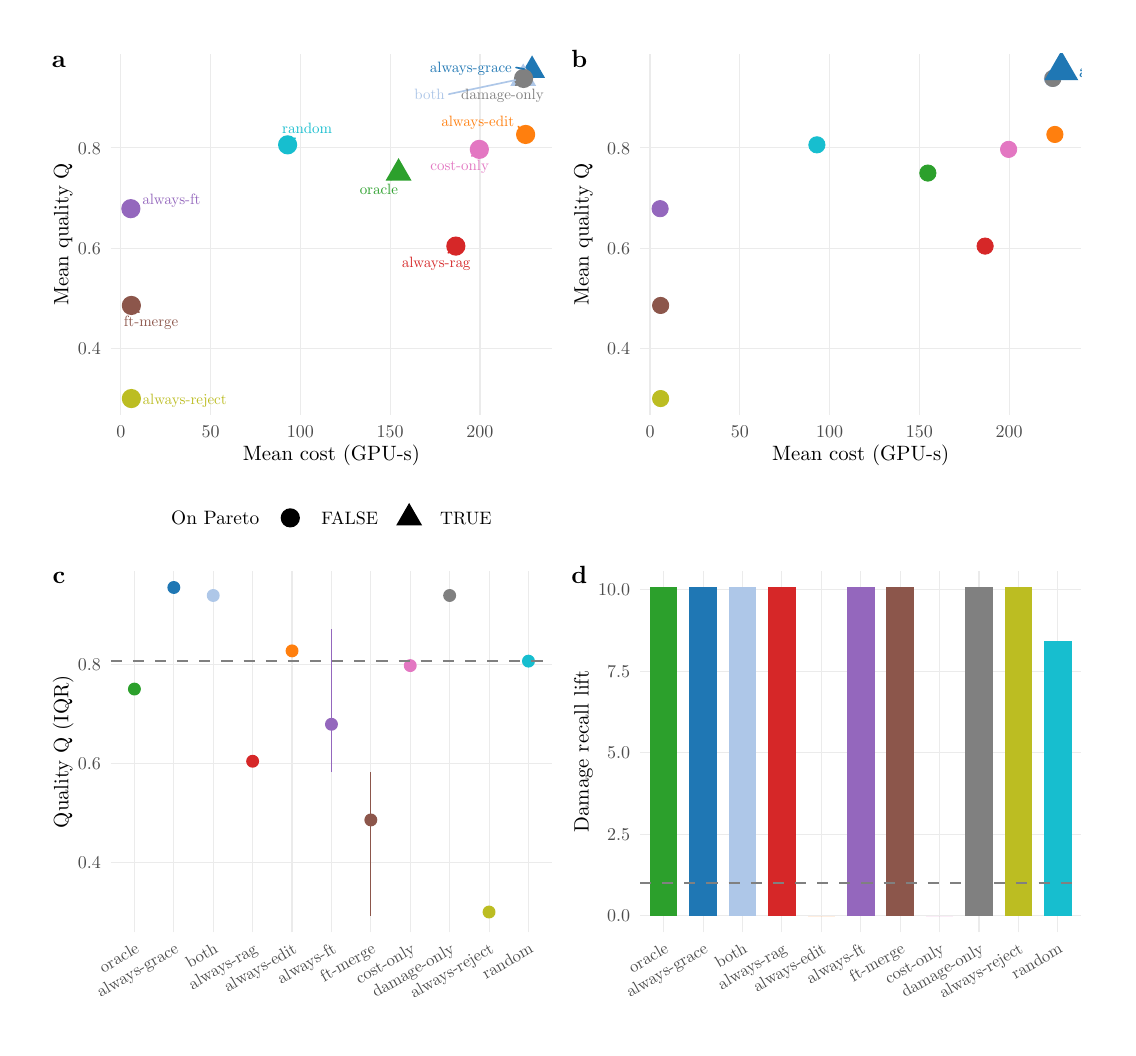
\begin{tikzpicture}[x=1pt,y=1pt]
\definecolor{fillColor}{RGB}{255,255,255}
\path[use as bounding box,fill=fillColor,fill opacity=0.00] (0,0) rectangle (390.26,361.35);
\begin{scope}
\path[clip] (  0.00,  0.00) rectangle (390.26,361.35);
\definecolor{drawColor}{RGB}{255,255,255}
\definecolor{fillColor}{RGB}{255,255,255}

\path[draw=drawColor,line width= 0.6pt,line join=round,line cap=round,fill=fillColor] (  0.00,  0.00) rectangle (390.26,361.35);
\end{scope}
\begin{scope}
\path[clip] (  5.50,168.99) rectangle (193.50,355.85);
\definecolor{fillColor}{RGB}{255,255,255}

\path[fill=fillColor] (  5.50,168.99) rectangle (193.50,355.85);
\end{scope}
\begin{scope}
\path[clip] (193.50,168.99) rectangle (384.76,355.85);
\definecolor{fillColor}{RGB}{255,255,255}

\path[fill=fillColor] (193.50,168.99) rectangle (384.76,355.85);
\end{scope}
\begin{scope}
\path[clip] (  5.50,  5.50) rectangle (193.50,168.99);
\definecolor{fillColor}{RGB}{255,255,255}

\path[fill=fillColor] (  5.50,  5.50) rectangle (193.50,168.99);
\end{scope}
\begin{scope}
\path[clip] (193.50,  5.50) rectangle (384.76,168.99);
\definecolor{fillColor}{RGB}{255,255,255}

\path[fill=fillColor] (193.50,  5.50) rectangle (384.76,168.99);
\end{scope}
\begin{scope}
\path[clip] ( 30.03,221.41) rectangle (189.50,351.85);
\definecolor{drawColor}{gray}{0.92}

\path[draw=drawColor,line width= 0.4pt,line join=round] ( 30.03,245.46) --
	(189.50,245.46);

\path[draw=drawColor,line width= 0.4pt,line join=round] ( 30.03,281.70) --
	(189.50,281.70);

\path[draw=drawColor,line width= 0.4pt,line join=round] ( 30.03,317.94) --
	(189.50,317.94);

\path[draw=drawColor,line width= 0.4pt,line join=round] ( 33.64,221.41) --
	( 33.64,351.85);

\path[draw=drawColor,line width= 0.4pt,line join=round] ( 66.09,221.41) --
	( 66.09,351.85);

\path[draw=drawColor,line width= 0.4pt,line join=round] ( 98.53,221.41) --
	( 98.53,351.85);

\path[draw=drawColor,line width= 0.4pt,line join=round] (130.98,221.41) --
	(130.98,351.85);

\path[draw=drawColor,line width= 0.4pt,line join=round] (163.43,221.41) --
	(163.43,351.85);
\definecolor{fillColor}{RGB}{44,160,44}

\path[fill=fillColor] (134.02,314.21) --
	(138.70,306.11) --
	(129.35,306.11) --
	cycle;
\definecolor{fillColor}{RGB}{31,119,180}

\path[fill=fillColor] (182.26,351.32) --
	(186.93,343.22) --
	(177.58,343.22) --
	cycle;
\definecolor{fillColor}{RGB}{174,199,232}

\path[fill=fillColor] (179.05,348.40) --
	(183.73,340.30) --
	(174.38,340.30) --
	cycle;
\definecolor{fillColor}{RGB}{214,39,40}

\path[fill=fillColor] (154.72,282.42) circle (  3.47);
\definecolor{fillColor}{RGB}{255,127,14}

\path[fill=fillColor] (179.93,322.76) circle (  3.47);
\definecolor{fillColor}{RGB}{148,103,189}

\path[fill=fillColor] ( 37.28,295.94) circle (  3.47);
\definecolor{fillColor}{RGB}{140,86,75}

\path[fill=fillColor] ( 37.47,260.97) circle (  3.47);
\definecolor{fillColor}{RGB}{227,119,194}

\path[fill=fillColor] (163.21,317.37) circle (  3.47);
\definecolor{fillColor}{gray}{0.50}

\path[fill=fillColor] (179.19,343.00) circle (  3.47);
\definecolor{fillColor}{RGB}{188,189,34}

\path[fill=fillColor] ( 37.47,227.33) circle (  3.47);
\definecolor{fillColor}{RGB}{23,190,207}

\path[fill=fillColor] ( 93.93,319.01) circle (  3.47);
\definecolor{drawColor}{RGB}{44,160,44}

\path[draw=drawColor,line width= 0.6pt,line join=round,line cap=round] (131.26,306.36) -- (131.87,306.90);
\definecolor{drawColor}{RGB}{31,119,180}

\path[draw=drawColor,line width= 0.6pt,line join=round,line cap=round] (176.46,346.95) -- (179.42,346.42);
\definecolor{drawColor}{RGB}{174,199,232}

\path[draw=drawColor,line width= 0.6pt,line join=round,line cap=round] (152.17,337.32) -- (176.24,342.40);
\definecolor{drawColor}{RGB}{214,39,40}

\path[draw=drawColor,line width= 0.6pt,line join=round,line cap=round] (151.94,279.96) -- (152.56,280.51);
\definecolor{drawColor}{RGB}{255,127,14}

\path[draw=drawColor,line width= 0.6pt,line join=round,line cap=round] (177.29,325.65) -- (177.99,324.88);
\definecolor{drawColor}{RGB}{148,103,189}

\path[draw=drawColor,line width= 0.6pt,line join=round,line cap=round] ( 39.91,297.80) -- ( 39.63,297.60);
\definecolor{drawColor}{RGB}{140,86,75}

\path[draw=drawColor,line width= 0.6pt,line join=round,line cap=round] ( 40.25,258.50) -- ( 39.62,259.06);
\definecolor{drawColor}{RGB}{227,119,194}

\path[draw=drawColor,line width= 0.6pt,line join=round,line cap=round] (160.46,314.94) -- (161.06,315.46);
\definecolor{drawColor}{gray}{0.50}

\path[draw=drawColor,line width= 0.6pt,line join=round,line cap=round] (176.37,340.52) -- (177.03,341.10);
\definecolor{drawColor}{RGB}{23,190,207}

\path[draw=drawColor,line width= 0.6pt,line join=round,line cap=round] ( 96.66,321.44) -- ( 96.08,320.92);
\definecolor{drawColor}{RGB}{44,160,44}

\node[text=drawColor,anchor=base,inner sep=0pt, outer sep=0pt, scale=  0.54] at (126.91,301.13) {oracle};
\definecolor{drawColor}{RGB}{31,119,180}

\node[text=drawColor,anchor=base,inner sep=0pt, outer sep=0pt, scale=  0.54] at (160.14,345.12) {always-grace};
\definecolor{drawColor}{RGB}{174,199,232}

\node[text=drawColor,anchor=base,inner sep=0pt, outer sep=0pt, scale=  0.54] at (145.19,335.37) {both};
\definecolor{drawColor}{RGB}{214,39,40}

\node[text=drawColor,anchor=base,inner sep=0pt, outer sep=0pt, scale=  0.54] at (147.60,274.73) {always-rag};
\definecolor{drawColor}{RGB}{255,127,14}

\node[text=drawColor,anchor=base,inner sep=0pt, outer sep=0pt, scale=  0.54] at (162.63,325.51) {always-edit};
\definecolor{drawColor}{RGB}{148,103,189}

\node[text=drawColor,anchor=base,inner sep=0pt, outer sep=0pt, scale=  0.54] at ( 51.94,297.51) {always-ft};
\definecolor{drawColor}{RGB}{140,86,75}

\node[text=drawColor,anchor=base,inner sep=0pt, outer sep=0pt, scale=  0.54] at ( 44.61,253.27) {ft-merge};
\definecolor{drawColor}{RGB}{227,119,194}

\node[text=drawColor,anchor=base,inner sep=0pt, outer sep=0pt, scale=  0.54] at (156.12,309.71) {cost-only};
\definecolor{drawColor}{gray}{0.50}

\node[text=drawColor,anchor=base,inner sep=0pt, outer sep=0pt, scale=  0.54] at (171.56,335.29) {damage-only};
\definecolor{drawColor}{RGB}{188,189,34}

\node[text=drawColor,anchor=base,inner sep=0pt, outer sep=0pt, scale=  0.54] at ( 56.74,225.27) {always-reject};
\definecolor{drawColor}{RGB}{23,190,207}

\node[text=drawColor,anchor=base,inner sep=0pt, outer sep=0pt, scale=  0.54] at (100.99,322.94) {random};
\end{scope}
\begin{scope}
\path[clip] (  0.00,  0.00) rectangle (390.26,361.35);
\definecolor{drawColor}{gray}{0.30}

\node[text=drawColor,anchor=base east,inner sep=0pt, outer sep=0pt, scale=  0.65] at ( 26.43,243.22) {0.4};

\node[text=drawColor,anchor=base east,inner sep=0pt, outer sep=0pt, scale=  0.65] at ( 26.43,279.46) {0.6};

\node[text=drawColor,anchor=base east,inner sep=0pt, outer sep=0pt, scale=  0.65] at ( 26.43,315.70) {0.8};
\end{scope}
\begin{scope}
\path[clip] (  0.00,  0.00) rectangle (390.26,361.35);
\definecolor{drawColor}{gray}{0.30}

\node[text=drawColor,anchor=base,inner sep=0pt, outer sep=0pt, scale=  0.65] at ( 33.64,213.33) {0};

\node[text=drawColor,anchor=base,inner sep=0pt, outer sep=0pt, scale=  0.65] at ( 66.09,213.33) {50};

\node[text=drawColor,anchor=base,inner sep=0pt, outer sep=0pt, scale=  0.65] at ( 98.53,213.33) {100};

\node[text=drawColor,anchor=base,inner sep=0pt, outer sep=0pt, scale=  0.65] at (130.98,213.33) {150};

\node[text=drawColor,anchor=base,inner sep=0pt, outer sep=0pt, scale=  0.65] at (163.43,213.33) {200};
\end{scope}
\begin{scope}
\path[clip] (  0.00,  0.00) rectangle (390.26,361.35);
\definecolor{drawColor}{RGB}{0,0,0}

\node[text=drawColor,anchor=base,inner sep=0pt, outer sep=0pt, scale=  0.75] at (109.77,204.90) {Mean cost (GPU-s)};
\end{scope}
\begin{scope}
\path[clip] (  0.00,  0.00) rectangle (390.26,361.35);
\definecolor{drawColor}{RGB}{0,0,0}

\node[text=drawColor,rotate= 90.00,anchor=base,inner sep=0pt, outer sep=0pt, scale=  0.75] at ( 14.67,286.63) {Mean quality Q};
\end{scope}
\begin{scope}
\path[clip] (  0.00,  0.00) rectangle (390.26,361.35);
\definecolor{drawColor}{RGB}{0,0,0}

\node[text=drawColor,anchor=base west,inner sep=0pt, outer sep=0pt, scale=  0.70] at ( 51.87,181.80) {On Pareto};
\end{scope}
\begin{scope}
\path[clip] (  0.00,  0.00) rectangle (390.26,361.35);
\definecolor{fillColor}{RGB}{0,0,0}

\path[fill=fillColor] ( 94.90,184.21) circle (  3.47);
\end{scope}
\begin{scope}
\path[clip] (  0.00,  0.00) rectangle (390.26,361.35);
\definecolor{fillColor}{RGB}{0,0,0}

\path[fill=fillColor] (137.84,189.61) --
	(142.52,181.52) --
	(133.17,181.52) --
	cycle;
\end{scope}
\begin{scope}
\path[clip] (  0.00,  0.00) rectangle (390.26,361.35);
\definecolor{drawColor}{RGB}{0,0,0}

\node[text=drawColor,anchor=base west,inner sep=0pt, outer sep=0pt, scale=  0.65] at (106.13,181.98) {FALSE};
\end{scope}
\begin{scope}
\path[clip] (  0.00,  0.00) rectangle (390.26,361.35);
\definecolor{drawColor}{RGB}{0,0,0}

\node[text=drawColor,anchor=base west,inner sep=0pt, outer sep=0pt, scale=  0.65] at (149.07,181.98) {TRUE};
\end{scope}
\begin{scope}
\path[clip] (  0.00,  0.00) rectangle (390.26,361.35);
\definecolor{drawColor}{RGB}{0,0,0}

\node[text=drawColor,anchor=base,inner sep=0pt, outer sep=0pt, scale=  0.90] at ( 11.30,346.96) {\bfseries a};
\end{scope}
\begin{scope}
\path[clip] (221.28,221.41) rectangle (380.76,351.85);
\definecolor{drawColor}{gray}{0.92}

\path[draw=drawColor,line width= 0.4pt,line join=round] (221.28,245.46) --
	(380.76,245.46);

\path[draw=drawColor,line width= 0.4pt,line join=round] (221.28,281.70) --
	(380.76,281.70);

\path[draw=drawColor,line width= 0.4pt,line join=round] (221.28,317.94) --
	(380.76,317.94);

\path[draw=drawColor,line width= 0.4pt,line join=round] (224.89,221.41) --
	(224.89,351.85);

\path[draw=drawColor,line width= 0.4pt,line join=round] (257.34,221.41) --
	(257.34,351.85);

\path[draw=drawColor,line width= 0.4pt,line join=round] (289.79,221.41) --
	(289.79,351.85);

\path[draw=drawColor,line width= 0.4pt,line join=round] (322.23,221.41) --
	(322.23,351.85);

\path[draw=drawColor,line width= 0.4pt,line join=round] (354.68,221.41) --
	(354.68,351.85);
\definecolor{drawColor}{RGB}{44,160,44}
\definecolor{fillColor}{RGB}{44,160,44}

\path[draw=drawColor,line width= 0.3pt,line join=round,line cap=round,fill=fillColor] (325.28,308.81) circle (  2.94);
\definecolor{drawColor}{RGB}{31,119,180}
\definecolor{fillColor}{RGB}{31,119,180}

\path[draw=drawColor,line width= 0.3pt,line join=round,line cap=round,fill=fillColor] (373.51,345.92) circle (  2.94);
\definecolor{drawColor}{RGB}{174,199,232}
\definecolor{fillColor}{RGB}{174,199,232}

\path[draw=drawColor,line width= 0.3pt,line join=round,line cap=round,fill=fillColor] (370.31,343.00) circle (  2.94);
\definecolor{drawColor}{RGB}{214,39,40}
\definecolor{fillColor}{RGB}{214,39,40}

\path[draw=drawColor,line width= 0.3pt,line join=round,line cap=round,fill=fillColor] (345.97,282.42) circle (  2.94);
\definecolor{drawColor}{RGB}{255,127,14}
\definecolor{fillColor}{RGB}{255,127,14}

\path[draw=drawColor,line width= 0.3pt,line join=round,line cap=round,fill=fillColor] (371.18,322.76) circle (  2.94);
\definecolor{drawColor}{RGB}{148,103,189}
\definecolor{fillColor}{RGB}{148,103,189}

\path[draw=drawColor,line width= 0.3pt,line join=round,line cap=round,fill=fillColor] (228.53,295.94) circle (  2.94);
\definecolor{drawColor}{RGB}{140,86,75}
\definecolor{fillColor}{RGB}{140,86,75}

\path[draw=drawColor,line width= 0.3pt,line join=round,line cap=round,fill=fillColor] (228.72,260.97) circle (  2.94);
\definecolor{drawColor}{RGB}{227,119,194}
\definecolor{fillColor}{RGB}{227,119,194}

\path[draw=drawColor,line width= 0.3pt,line join=round,line cap=round,fill=fillColor] (354.46,317.37) circle (  2.94);
\definecolor{drawColor}{gray}{0.50}
\definecolor{fillColor}{gray}{0.50}

\path[draw=drawColor,line width= 0.3pt,line join=round,line cap=round,fill=fillColor] (370.45,343.00) circle (  2.94);
\definecolor{drawColor}{RGB}{188,189,34}
\definecolor{fillColor}{RGB}{188,189,34}

\path[draw=drawColor,line width= 0.3pt,line join=round,line cap=round,fill=fillColor] (228.72,227.33) circle (  2.94);
\definecolor{drawColor}{RGB}{23,190,207}
\definecolor{fillColor}{RGB}{23,190,207}

\path[draw=drawColor,line width= 0.3pt,line join=round,line cap=round,fill=fillColor] (285.18,319.01) circle (  2.94);
\definecolor{fillColor}{RGB}{31,119,180}

\path[fill=fillColor] (373.51,352.98) --
	(379.63,342.39) --
	(367.39,342.39) --
	cycle;
\definecolor{drawColor}{RGB}{31,119,180}

\node[text=drawColor,anchor=base west,inner sep=0pt, outer sep=0pt, scale=  0.71] at (379.83,343.47) {always\_grace};
\end{scope}
\begin{scope}
\path[clip] (  0.00,  0.00) rectangle (390.26,361.35);
\definecolor{drawColor}{gray}{0.30}

\node[text=drawColor,anchor=base east,inner sep=0pt, outer sep=0pt, scale=  0.65] at (217.68,243.22) {0.4};

\node[text=drawColor,anchor=base east,inner sep=0pt, outer sep=0pt, scale=  0.65] at (217.68,279.46) {0.6};

\node[text=drawColor,anchor=base east,inner sep=0pt, outer sep=0pt, scale=  0.65] at (217.68,315.70) {0.8};
\end{scope}
\begin{scope}
\path[clip] (  0.00,  0.00) rectangle (390.26,361.35);
\definecolor{drawColor}{gray}{0.30}

\node[text=drawColor,anchor=base,inner sep=0pt, outer sep=0pt, scale=  0.65] at (224.89,213.33) {0};

\node[text=drawColor,anchor=base,inner sep=0pt, outer sep=0pt, scale=  0.65] at (257.34,213.33) {50};

\node[text=drawColor,anchor=base,inner sep=0pt, outer sep=0pt, scale=  0.65] at (289.79,213.33) {100};

\node[text=drawColor,anchor=base,inner sep=0pt, outer sep=0pt, scale=  0.65] at (322.23,213.33) {150};

\node[text=drawColor,anchor=base,inner sep=0pt, outer sep=0pt, scale=  0.65] at (354.68,213.33) {200};
\end{scope}
\begin{scope}
\path[clip] (  0.00,  0.00) rectangle (390.26,361.35);
\definecolor{drawColor}{RGB}{0,0,0}

\node[text=drawColor,anchor=base,inner sep=0pt, outer sep=0pt, scale=  0.75] at (301.02,204.90) {Mean cost (GPU-s)};
\end{scope}
\begin{scope}
\path[clip] (  0.00,  0.00) rectangle (390.26,361.35);
\definecolor{drawColor}{RGB}{0,0,0}

\node[text=drawColor,rotate= 90.00,anchor=base,inner sep=0pt, outer sep=0pt, scale=  0.75] at (202.67,286.63) {Mean quality Q};
\end{scope}
\begin{scope}
\path[clip] (  0.00,  0.00) rectangle (390.26,361.35);
\definecolor{drawColor}{RGB}{0,0,0}

\node[text=drawColor,anchor=base,inner sep=0pt, outer sep=0pt, scale=  0.90] at (199.34,346.96) {\bfseries b};
\end{scope}
\begin{scope}
\path[clip] ( 30.03, 34.54) rectangle (189.50,164.99);
\definecolor{drawColor}{gray}{0.92}

\path[draw=drawColor,line width= 0.4pt,line join=round] ( 30.03, 59.71) --
	(189.50, 59.71);

\path[draw=drawColor,line width= 0.4pt,line join=round] ( 30.03, 95.55) --
	(189.50, 95.55);

\path[draw=drawColor,line width= 0.4pt,line join=round] ( 30.03,131.39) --
	(189.50,131.39);

\path[draw=drawColor,line width= 0.4pt,line join=round] ( 38.57, 34.54) --
	( 38.57,164.99);

\path[draw=drawColor,line width= 0.4pt,line join=round] ( 52.81, 34.54) --
	( 52.81,164.99);

\path[draw=drawColor,line width= 0.4pt,line join=round] ( 67.05, 34.54) --
	( 67.05,164.99);

\path[draw=drawColor,line width= 0.4pt,line join=round] ( 81.29, 34.54) --
	( 81.29,164.99);

\path[draw=drawColor,line width= 0.4pt,line join=round] ( 95.53, 34.54) --
	( 95.53,164.99);

\path[draw=drawColor,line width= 0.4pt,line join=round] (109.77, 34.54) --
	(109.77,164.99);

\path[draw=drawColor,line width= 0.4pt,line join=round] (124.00, 34.54) --
	(124.00,164.99);

\path[draw=drawColor,line width= 0.4pt,line join=round] (138.24, 34.54) --
	(138.24,164.99);

\path[draw=drawColor,line width= 0.4pt,line join=round] (152.48, 34.54) --
	(152.48,164.99);

\path[draw=drawColor,line width= 0.4pt,line join=round] (166.72, 34.54) --
	(166.72,164.99);

\path[draw=drawColor,line width= 0.4pt,line join=round] (180.96, 34.54) --
	(180.96,164.99);
\definecolor{drawColor}{RGB}{44,160,44}

\path[draw=drawColor,line width= 0.4pt,line join=round] ( 38.57,122.14) -- ( 38.57,122.57);
\definecolor{drawColor}{RGB}{31,119,180}

\path[draw=drawColor,line width= 0.4pt,line join=round] ( 52.81,159.06) -- ( 52.81,159.06);
\definecolor{drawColor}{RGB}{174,199,232}

\path[draw=drawColor,line width= 0.4pt,line join=round] ( 67.05,155.00) -- ( 67.05,158.40);
\definecolor{drawColor}{RGB}{214,39,40}

\path[draw=drawColor,line width= 0.4pt,line join=round] ( 81.29, 96.27) -- ( 81.29, 96.27);
\definecolor{drawColor}{RGB}{255,127,14}

\path[draw=drawColor,line width= 0.4pt,line join=round] ( 95.53,135.00) -- ( 95.53,137.88);
\definecolor{drawColor}{RGB}{148,103,189}

\path[draw=drawColor,line width= 0.4pt,line join=round] (109.77, 92.34) -- (109.77,144.22);
\definecolor{drawColor}{RGB}{140,86,75}

\path[draw=drawColor,line width= 0.4pt,line join=round] (124.00, 40.47) -- (124.00, 92.36);
\definecolor{drawColor}{RGB}{227,119,194}

\path[draw=drawColor,line width= 0.4pt,line join=round] (138.24,129.24) -- (138.24,132.62);
\definecolor{drawColor}{gray}{0.50}

\path[draw=drawColor,line width= 0.4pt,line join=round] (152.48,155.00) -- (152.48,158.40);
\definecolor{drawColor}{RGB}{188,189,34}

\path[draw=drawColor,line width= 0.4pt,line join=round] (166.72, 41.79) -- (166.72, 41.79);
\definecolor{drawColor}{RGB}{23,190,207}

\path[draw=drawColor,line width= 0.4pt,line join=round] (180.96,132.12) -- (180.96,133.00);
\definecolor{drawColor}{RGB}{44,160,44}
\definecolor{fillColor}{RGB}{44,160,44}

\path[draw=drawColor,line width= 0.5pt,line join=round,line cap=round,fill=fillColor] ( 38.57,122.36) circle (  2.08);
\definecolor{drawColor}{RGB}{31,119,180}
\definecolor{fillColor}{RGB}{31,119,180}

\path[draw=drawColor,line width= 0.5pt,line join=round,line cap=round,fill=fillColor] ( 52.81,159.06) circle (  2.08);
\definecolor{drawColor}{RGB}{174,199,232}
\definecolor{fillColor}{RGB}{174,199,232}

\path[draw=drawColor,line width= 0.5pt,line join=round,line cap=round,fill=fillColor] ( 67.05,156.17) circle (  2.08);
\definecolor{drawColor}{RGB}{214,39,40}
\definecolor{fillColor}{RGB}{214,39,40}

\path[draw=drawColor,line width= 0.5pt,line join=round,line cap=round,fill=fillColor] ( 81.29, 96.27) circle (  2.08);
\definecolor{drawColor}{RGB}{255,127,14}
\definecolor{fillColor}{RGB}{255,127,14}

\path[draw=drawColor,line width= 0.5pt,line join=round,line cap=round,fill=fillColor] ( 95.53,136.15) circle (  2.08);
\definecolor{drawColor}{RGB}{148,103,189}
\definecolor{fillColor}{RGB}{148,103,189}

\path[draw=drawColor,line width= 0.5pt,line join=round,line cap=round,fill=fillColor] (109.77,109.63) circle (  2.08);
\definecolor{drawColor}{RGB}{140,86,75}
\definecolor{fillColor}{RGB}{140,86,75}

\path[draw=drawColor,line width= 0.5pt,line join=round,line cap=round,fill=fillColor] (124.00, 75.06) circle (  2.08);
\definecolor{drawColor}{RGB}{227,119,194}
\definecolor{fillColor}{RGB}{227,119,194}

\path[draw=drawColor,line width= 0.5pt,line join=round,line cap=round,fill=fillColor] (138.24,130.83) circle (  2.08);
\definecolor{drawColor}{gray}{0.50}
\definecolor{fillColor}{gray}{0.50}

\path[draw=drawColor,line width= 0.5pt,line join=round,line cap=round,fill=fillColor] (152.48,156.17) circle (  2.08);
\definecolor{drawColor}{RGB}{188,189,34}
\definecolor{fillColor}{RGB}{188,189,34}

\path[draw=drawColor,line width= 0.5pt,line join=round,line cap=round,fill=fillColor] (166.72, 41.79) circle (  2.08);
\definecolor{drawColor}{RGB}{23,190,207}
\definecolor{fillColor}{RGB}{23,190,207}

\path[draw=drawColor,line width= 0.5pt,line join=round,line cap=round,fill=fillColor] (180.96,132.45) circle (  2.08);
\definecolor{drawColor}{gray}{0.50}

\path[draw=drawColor,line width= 0.5pt,dash pattern=on 4pt off 4pt ,line join=round] ( 30.03,132.45) -- (189.50,132.45);
\end{scope}
\begin{scope}
\path[clip] (  0.00,  0.00) rectangle (390.26,361.35);
\definecolor{drawColor}{gray}{0.30}

\node[text=drawColor,anchor=base east,inner sep=0pt, outer sep=0pt, scale=  0.65] at ( 26.43, 57.47) {0.4};

\node[text=drawColor,anchor=base east,inner sep=0pt, outer sep=0pt, scale=  0.65] at ( 26.43, 93.31) {0.6};

\node[text=drawColor,anchor=base east,inner sep=0pt, outer sep=0pt, scale=  0.65] at ( 26.43,129.15) {0.8};
\end{scope}
\begin{scope}
\path[clip] (  0.00,  0.00) rectangle (390.26,361.35);
\definecolor{drawColor}{gray}{0.30}

\node[text=drawColor,rotate= 30.00,anchor=base east,inner sep=0pt, outer sep=0pt, scale=  0.60] at ( 40.64, 27.36) {oracle};

\node[text=drawColor,rotate= 30.00,anchor=base east,inner sep=0pt, outer sep=0pt, scale=  0.60] at ( 54.88, 27.36) {always-grace};

\node[text=drawColor,rotate= 30.00,anchor=base east,inner sep=0pt, outer sep=0pt, scale=  0.60] at ( 69.11, 27.36) {both};

\node[text=drawColor,rotate= 30.00,anchor=base east,inner sep=0pt, outer sep=0pt, scale=  0.60] at ( 83.35, 27.36) {always-rag};

\node[text=drawColor,rotate= 30.00,anchor=base east,inner sep=0pt, outer sep=0pt, scale=  0.60] at ( 97.59, 27.36) {always-edit};

\node[text=drawColor,rotate= 30.00,anchor=base east,inner sep=0pt, outer sep=0pt, scale=  0.60] at (111.83, 27.36) {always-ft};

\node[text=drawColor,rotate= 30.00,anchor=base east,inner sep=0pt, outer sep=0pt, scale=  0.60] at (126.07, 27.36) {ft-merge};

\node[text=drawColor,rotate= 30.00,anchor=base east,inner sep=0pt, outer sep=0pt, scale=  0.60] at (140.31, 27.36) {cost-only};

\node[text=drawColor,rotate= 30.00,anchor=base east,inner sep=0pt, outer sep=0pt, scale=  0.60] at (154.55, 27.36) {damage-only};

\node[text=drawColor,rotate= 30.00,anchor=base east,inner sep=0pt, outer sep=0pt, scale=  0.60] at (168.79, 27.36) {always-reject};

\node[text=drawColor,rotate= 30.00,anchor=base east,inner sep=0pt, outer sep=0pt, scale=  0.60] at (183.03, 27.36) {random};
\end{scope}
\begin{scope}
\path[clip] (  0.00,  0.00) rectangle (390.26,361.35);
\definecolor{drawColor}{RGB}{0,0,0}

\node[text=drawColor,rotate= 90.00,anchor=base,inner sep=0pt, outer sep=0pt, scale=  0.75] at ( 14.67, 99.77) {Quality Q (IQR)};
\end{scope}
\begin{scope}
\path[clip] (  0.00,  0.00) rectangle (390.26,361.35);
\definecolor{drawColor}{RGB}{0,0,0}

\node[text=drawColor,anchor=base,inner sep=0pt, outer sep=0pt, scale=  0.90] at ( 11.30,160.33) {\bfseries c};
\end{scope}
\begin{scope}
\path[clip] (221.28, 34.54) rectangle (380.76,164.99);
\definecolor{drawColor}{gray}{0.92}

\path[draw=drawColor,line width= 0.4pt,line join=round] (221.28, 40.47) --
	(380.76, 40.47);

\path[draw=drawColor,line width= 0.4pt,line join=round] (221.28, 69.91) --
	(380.76, 69.91);

\path[draw=drawColor,line width= 0.4pt,line join=round] (221.28, 99.35) --
	(380.76, 99.35);

\path[draw=drawColor,line width= 0.4pt,line join=round] (221.28,128.79) --
	(380.76,128.79);

\path[draw=drawColor,line width= 0.4pt,line join=round] (221.28,158.23) --
	(380.76,158.23);

\path[draw=drawColor,line width= 0.4pt,line join=round] (229.82, 34.54) --
	(229.82,164.99);

\path[draw=drawColor,line width= 0.4pt,line join=round] (244.06, 34.54) --
	(244.06,164.99);

\path[draw=drawColor,line width= 0.4pt,line join=round] (258.30, 34.54) --
	(258.30,164.99);

\path[draw=drawColor,line width= 0.4pt,line join=round] (272.54, 34.54) --
	(272.54,164.99);

\path[draw=drawColor,line width= 0.4pt,line join=round] (286.78, 34.54) --
	(286.78,164.99);

\path[draw=drawColor,line width= 0.4pt,line join=round] (301.02, 34.54) --
	(301.02,164.99);

\path[draw=drawColor,line width= 0.4pt,line join=round] (315.26, 34.54) --
	(315.26,164.99);

\path[draw=drawColor,line width= 0.4pt,line join=round] (329.50, 34.54) --
	(329.50,164.99);

\path[draw=drawColor,line width= 0.4pt,line join=round] (343.74, 34.54) --
	(343.74,164.99);

\path[draw=drawColor,line width= 0.4pt,line join=round] (357.98, 34.54) --
	(357.98,164.99);

\path[draw=drawColor,line width= 0.4pt,line join=round] (372.21, 34.54) --
	(372.21,164.99);
\definecolor{fillColor}{RGB}{44,160,44}

\path[fill=fillColor] (224.84, 40.47) rectangle (234.81,159.06);
\definecolor{fillColor}{RGB}{31,119,180}

\path[fill=fillColor] (239.08, 40.47) rectangle (249.05,159.06);
\definecolor{fillColor}{RGB}{174,199,232}

\path[fill=fillColor] (253.32, 40.47) rectangle (263.29,159.06);
\definecolor{fillColor}{RGB}{214,39,40}

\path[fill=fillColor] (267.56, 40.47) rectangle (277.52,159.06);
\definecolor{fillColor}{RGB}{255,127,14}

\path[fill=fillColor] (281.80, 40.47) rectangle (291.76, 40.47);
\definecolor{fillColor}{RGB}{148,103,189}

\path[fill=fillColor] (296.04, 40.47) rectangle (306.00,159.06);
\definecolor{fillColor}{RGB}{140,86,75}

\path[fill=fillColor] (310.27, 40.47) rectangle (320.24,159.06);
\definecolor{fillColor}{RGB}{227,119,194}

\path[fill=fillColor] (324.51, 40.47) rectangle (334.48, 40.47);
\definecolor{fillColor}{gray}{0.50}

\path[fill=fillColor] (338.75, 40.47) rectangle (348.72,159.06);
\definecolor{fillColor}{RGB}{188,189,34}

\path[fill=fillColor] (352.99, 40.47) rectangle (362.96,159.06);
\definecolor{fillColor}{RGB}{23,190,207}

\path[fill=fillColor] (367.23, 40.47) rectangle (377.20,139.86);
\definecolor{drawColor}{gray}{0.50}

\path[draw=drawColor,line width= 0.5pt,dash pattern=on 4pt off 4pt ,line join=round] (221.28, 52.25) -- (380.76, 52.25);
\end{scope}
\begin{scope}
\path[clip] (  0.00,  0.00) rectangle (390.26,361.35);
\definecolor{drawColor}{gray}{0.30}

\node[text=drawColor,anchor=base east,inner sep=0pt, outer sep=0pt, scale=  0.65] at (217.68, 38.23) {0.0};

\node[text=drawColor,anchor=base east,inner sep=0pt, outer sep=0pt, scale=  0.65] at (217.68, 67.67) {2.5};

\node[text=drawColor,anchor=base east,inner sep=0pt, outer sep=0pt, scale=  0.65] at (217.68, 97.11) {5.0};

\node[text=drawColor,anchor=base east,inner sep=0pt, outer sep=0pt, scale=  0.65] at (217.68,126.55) {7.5};

\node[text=drawColor,anchor=base east,inner sep=0pt, outer sep=0pt, scale=  0.65] at (217.68,155.99) {10.0};
\end{scope}
\begin{scope}
\path[clip] (  0.00,  0.00) rectangle (390.26,361.35);
\definecolor{drawColor}{gray}{0.30}

\node[text=drawColor,rotate= 30.00,anchor=base east,inner sep=0pt, outer sep=0pt, scale=  0.60] at (231.89, 27.36) {oracle};

\node[text=drawColor,rotate= 30.00,anchor=base east,inner sep=0pt, outer sep=0pt, scale=  0.60] at (246.13, 27.36) {always-grace};

\node[text=drawColor,rotate= 30.00,anchor=base east,inner sep=0pt, outer sep=0pt, scale=  0.60] at (260.37, 27.36) {both};

\node[text=drawColor,rotate= 30.00,anchor=base east,inner sep=0pt, outer sep=0pt, scale=  0.60] at (274.61, 27.36) {always-rag};

\node[text=drawColor,rotate= 30.00,anchor=base east,inner sep=0pt, outer sep=0pt, scale=  0.60] at (288.85, 27.36) {always-edit};

\node[text=drawColor,rotate= 30.00,anchor=base east,inner sep=0pt, outer sep=0pt, scale=  0.60] at (303.09, 27.36) {always-ft};

\node[text=drawColor,rotate= 30.00,anchor=base east,inner sep=0pt, outer sep=0pt, scale=  0.60] at (317.32, 27.36) {ft-merge};

\node[text=drawColor,rotate= 30.00,anchor=base east,inner sep=0pt, outer sep=0pt, scale=  0.60] at (331.56, 27.36) {cost-only};

\node[text=drawColor,rotate= 30.00,anchor=base east,inner sep=0pt, outer sep=0pt, scale=  0.60] at (345.80, 27.36) {damage-only};

\node[text=drawColor,rotate= 30.00,anchor=base east,inner sep=0pt, outer sep=0pt, scale=  0.60] at (360.04, 27.36) {always-reject};

\node[text=drawColor,rotate= 30.00,anchor=base east,inner sep=0pt, outer sep=0pt, scale=  0.60] at (374.28, 27.36) {random};
\end{scope}
\begin{scope}
\path[clip] (  0.00,  0.00) rectangle (390.26,361.35);
\definecolor{drawColor}{RGB}{0,0,0}

\node[text=drawColor,rotate= 90.00,anchor=base,inner sep=0pt, outer sep=0pt, scale=  0.75] at (202.67, 99.77) {Damage recall lift};
\end{scope}
\begin{scope}
\path[clip] (  0.00,  0.00) rectangle (390.26,361.35);
\definecolor{drawColor}{RGB}{0,0,0}

\node[text=drawColor,anchor=base,inner sep=0pt, outer sep=0pt, scale=  0.90] at (199.34,160.33) {\bfseries d};
\end{scope}
\end{tikzpicture}
